% 从 Xelatex/ 目录编译时的路径；从仓库根编译请去掉 ../。
% 导言区需要 \usepackage{graphicx}。按需要选用以下片段，不必全部插入。

\begin{figure}[htbp]
  \centering
  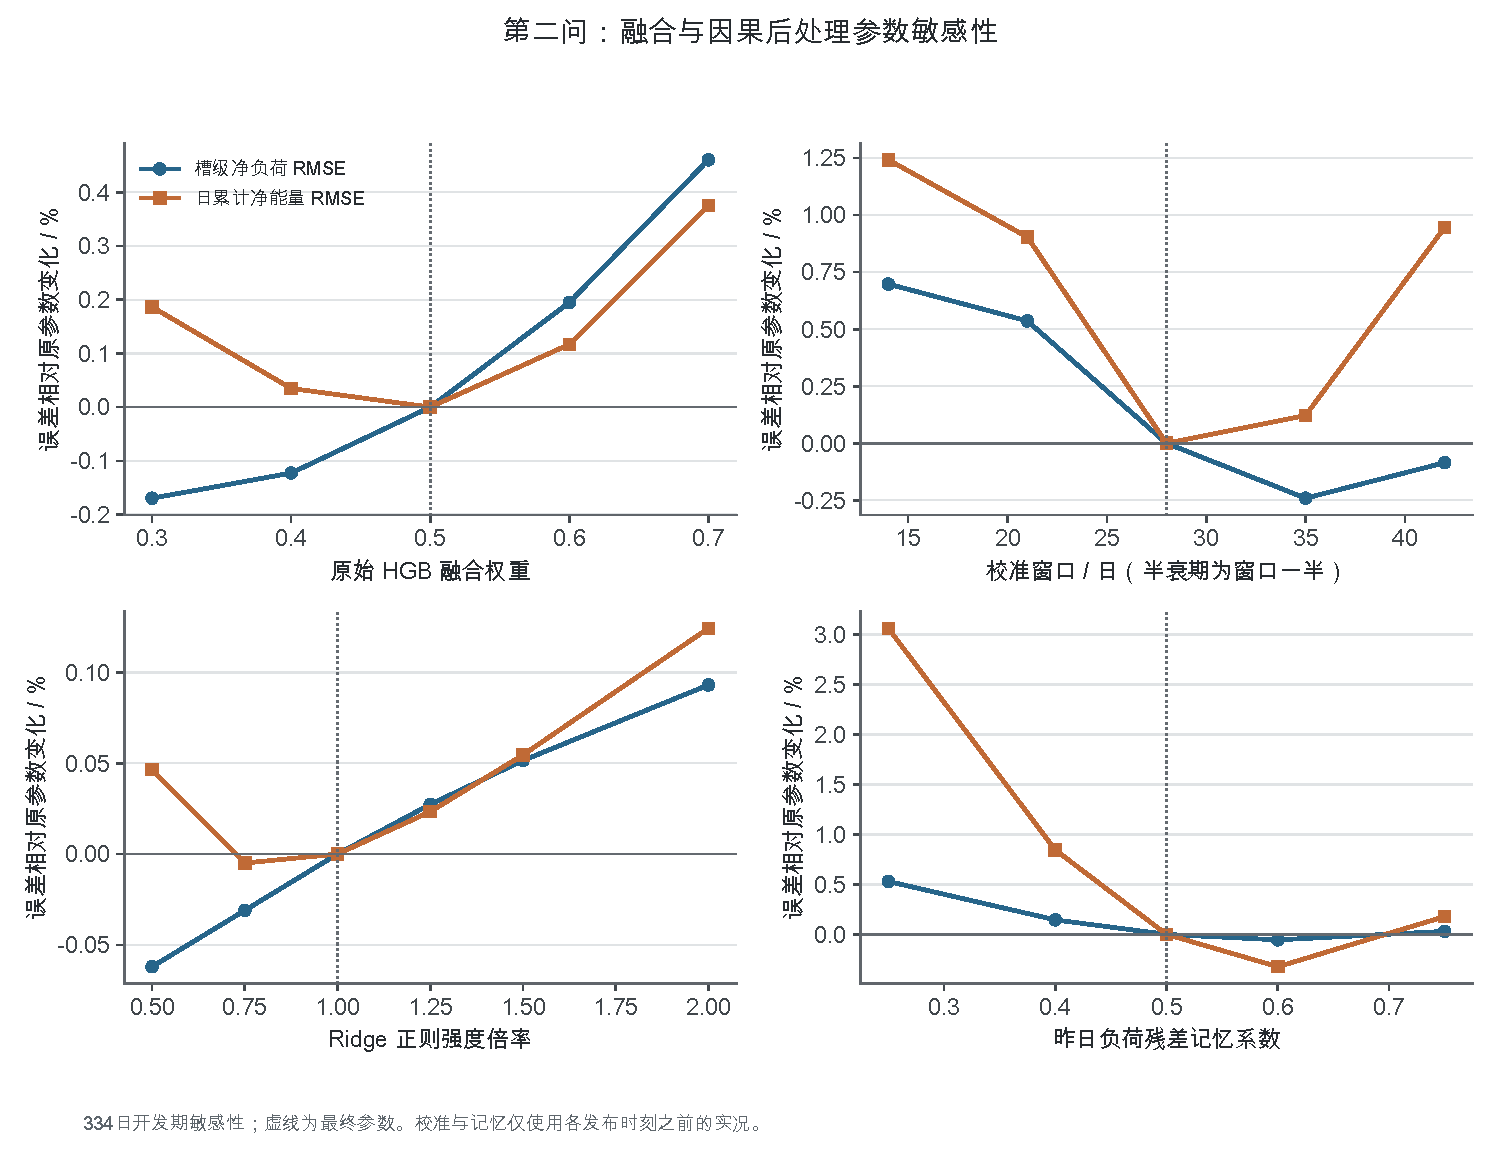
\includegraphics[width=0.96\linewidth]{../paper/figures/exp008_robustness/01_forecast_sensitivity.pdf}
  \caption{第二问：融合与因果后处理参数敏感性}
  \label{fig:exp008-01_forecast_sensitivity}
\end{figure}

\begin{figure}[htbp]
  \centering
  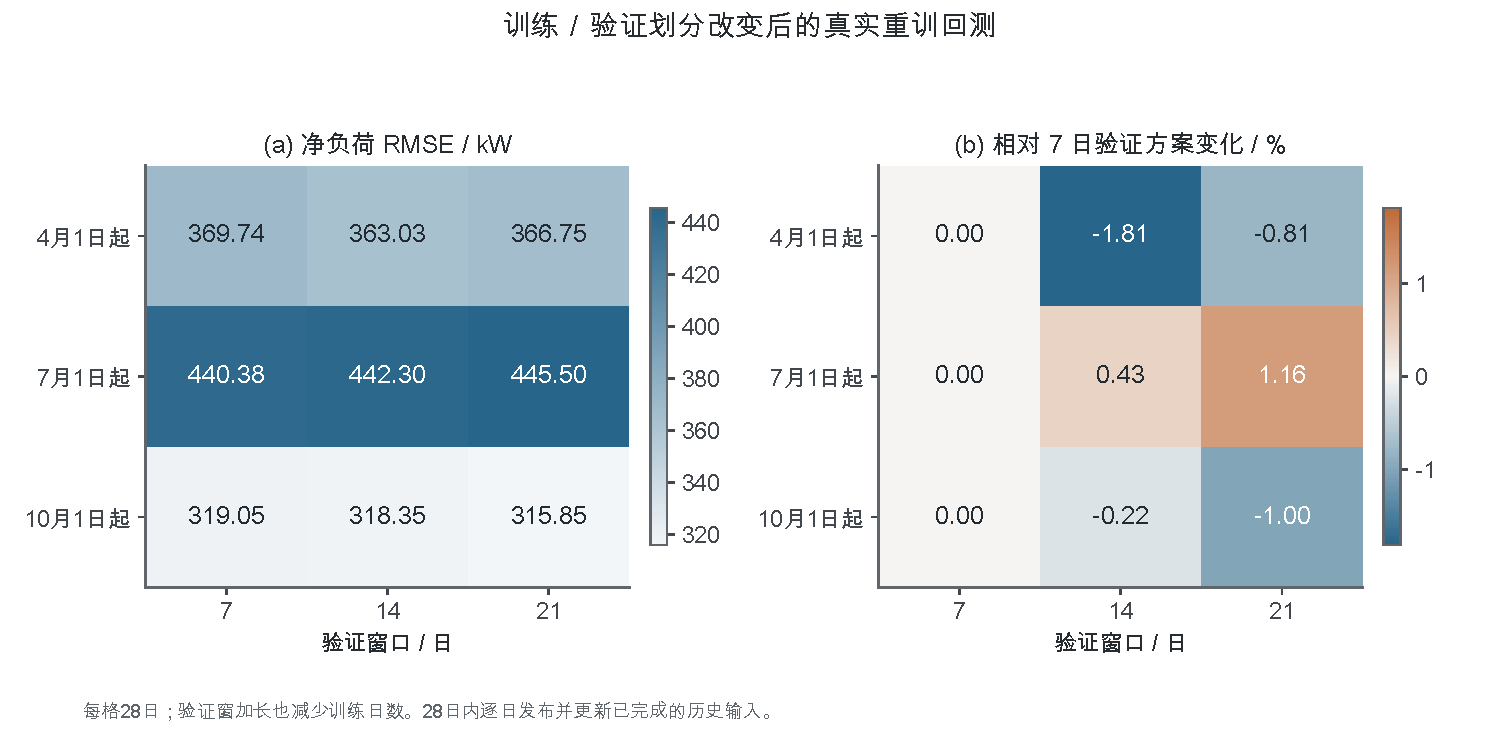
\includegraphics[width=0.96\linewidth]{../paper/figures/exp008_robustness/02_temporal_cv.pdf}
  \caption{训练／验证划分改变后的真实重训回测}
  \label{fig:exp008-02_temporal_cv}
\end{figure}

\begin{figure}[htbp]
  \centering
  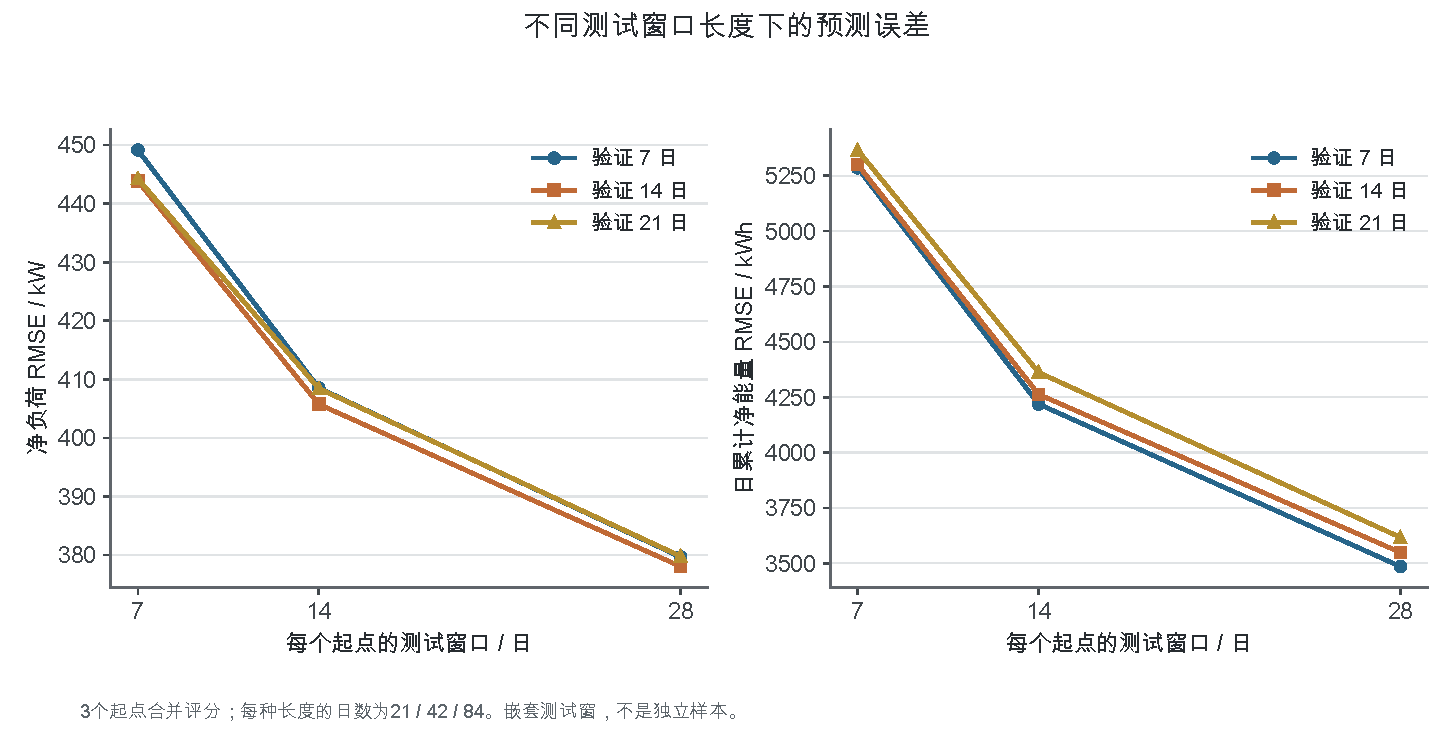
\includegraphics[width=0.96\linewidth]{../paper/figures/exp008_robustness/03_test_window.pdf}
  \caption{不同测试窗口长度下的预测误差}
  \label{fig:exp008-03_test_window}
\end{figure}

\begin{figure}[htbp]
  \centering
  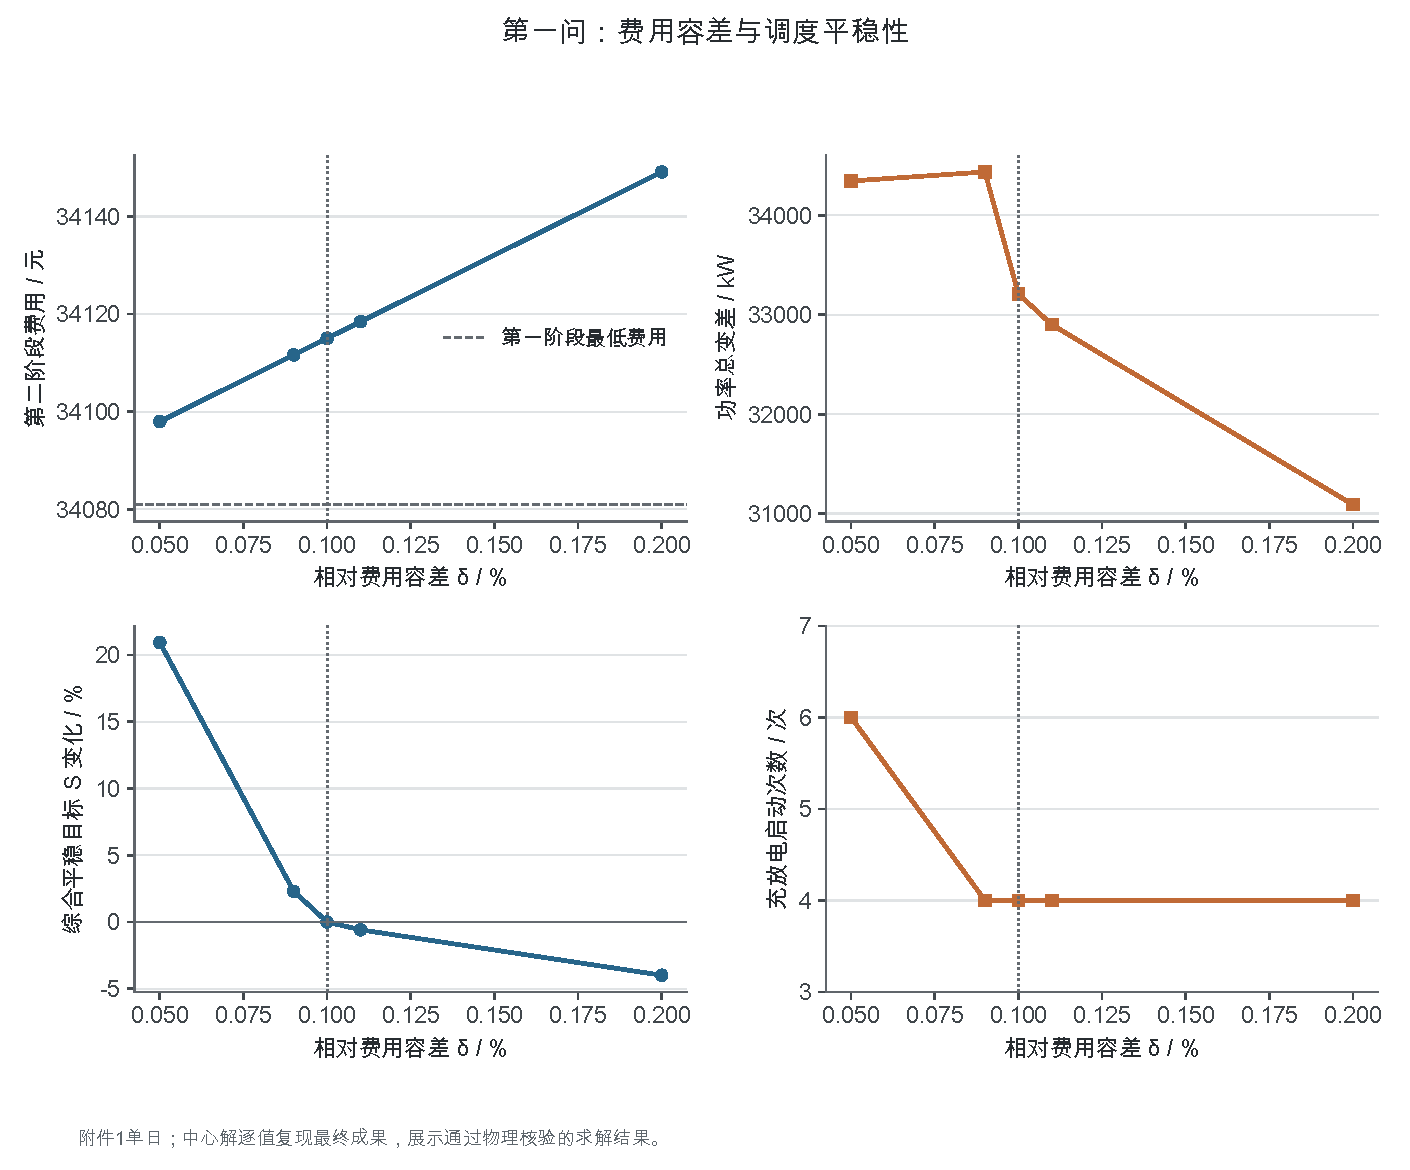
\includegraphics[width=0.96\linewidth]{../paper/figures/exp008_robustness/04_q1_budget.pdf}
  \caption{第一问：费用容差与调度平稳性}
  \label{fig:exp008-04_q1_budget}
\end{figure}

\begin{figure}[htbp]
  \centering
  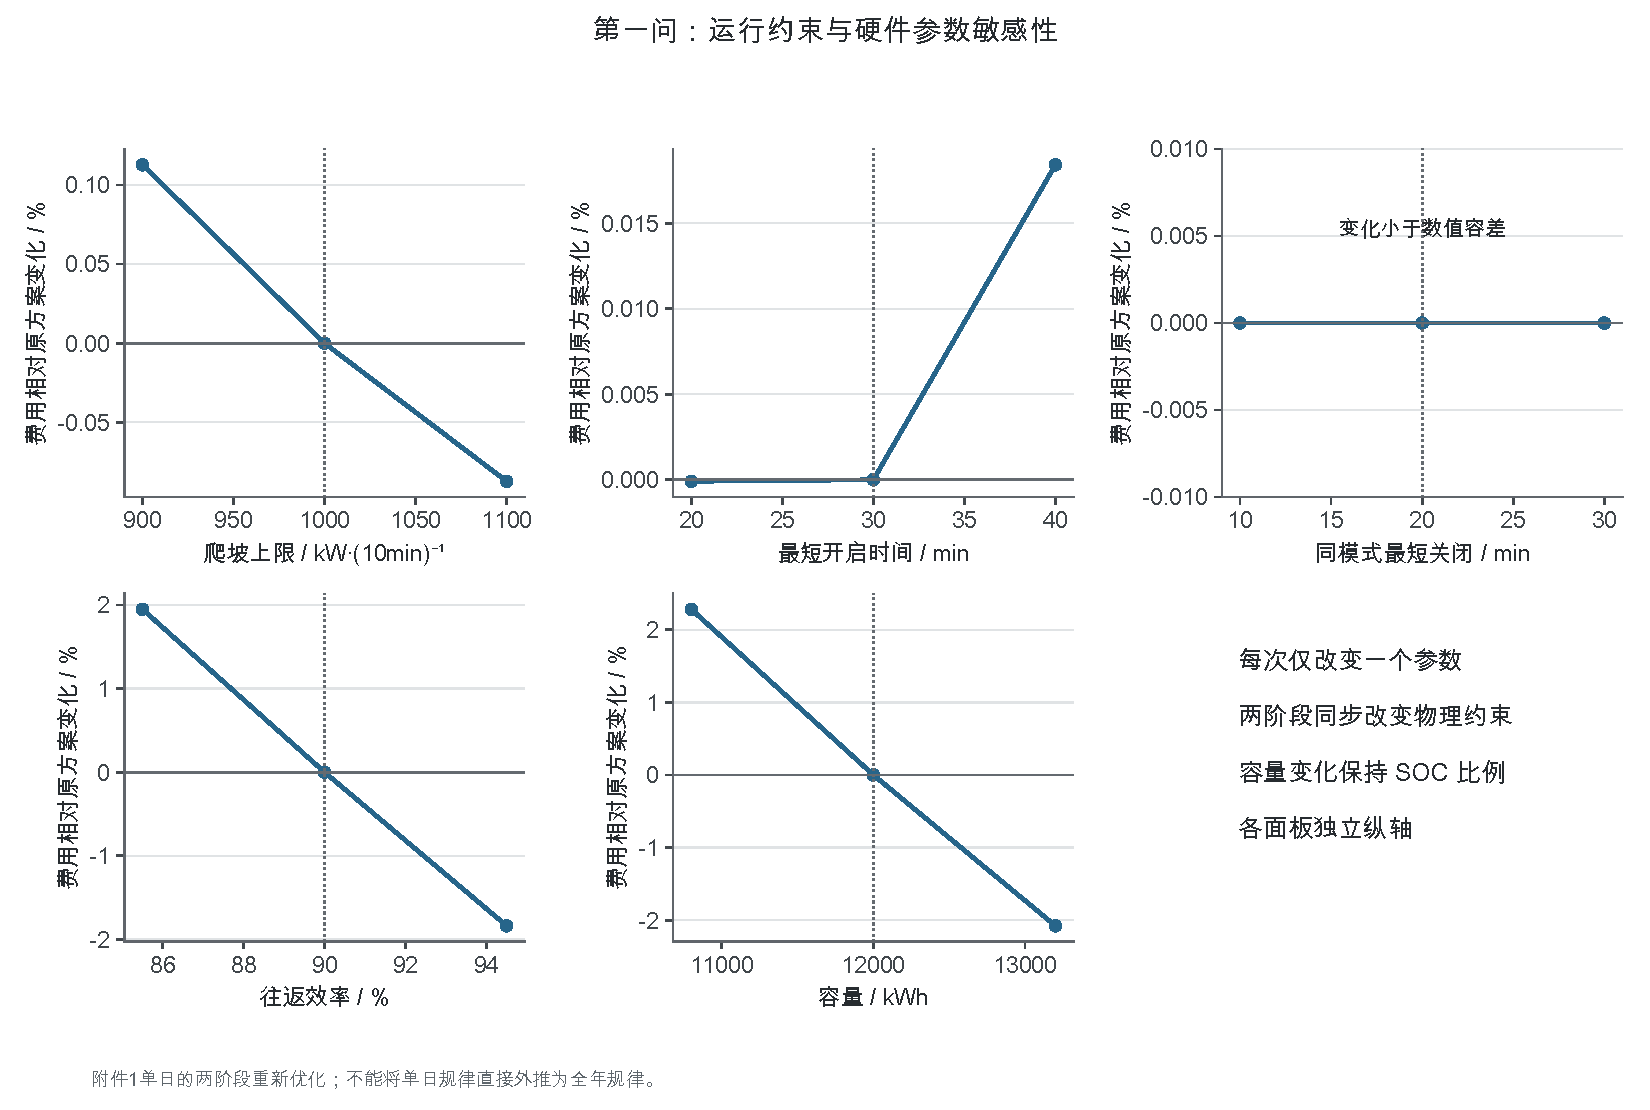
\includegraphics[width=0.96\linewidth]{../paper/figures/exp008_robustness/05_q1_parameters.pdf}
  \caption{第一问：运行约束与硬件参数敏感性}
  \label{fig:exp008-05_q1_parameters}
\end{figure}

\begin{figure}[htbp]
  \centering
  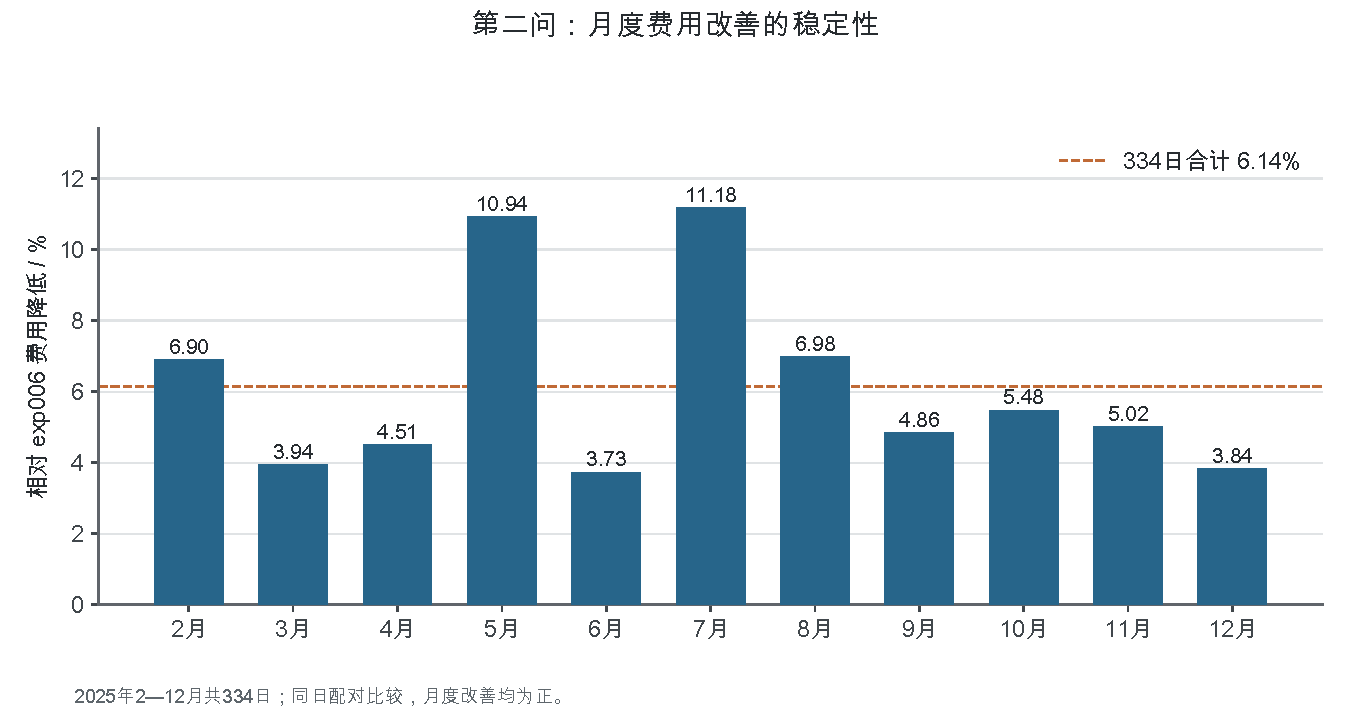
\includegraphics[width=0.96\linewidth]{../paper/figures/exp008_robustness/06_monthly_saving.pdf}
  \caption{第二问：月度费用改善的稳定性}
  \label{fig:exp008-06_monthly_saving}
\end{figure}

\begin{figure}[htbp]
  \centering
  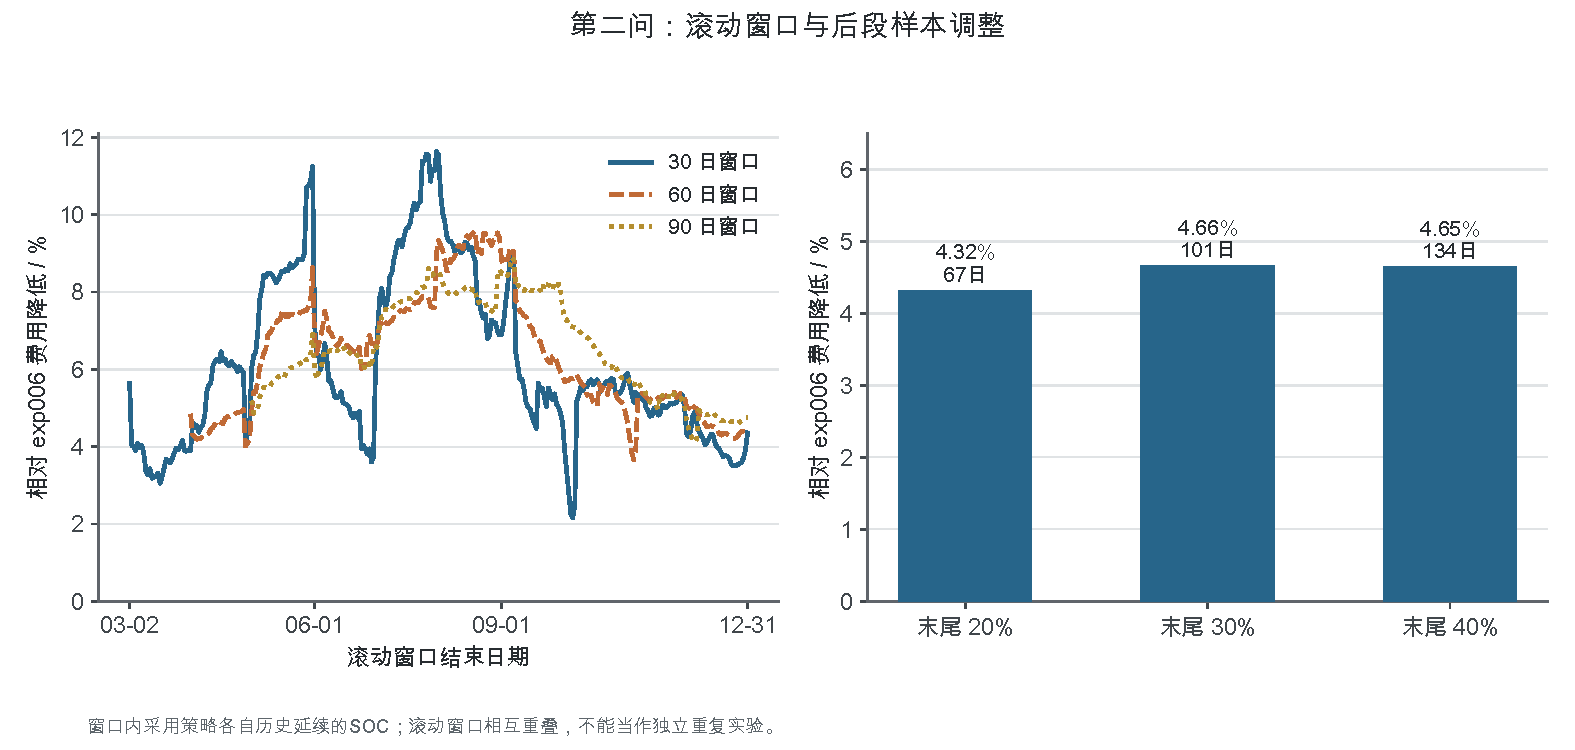
\includegraphics[width=0.96\linewidth]{../paper/figures/exp008_robustness/07_rolling_and_tail.pdf}
  \caption{第二问：滚动窗口与后段样本调整}
  \label{fig:exp008-07_rolling_and_tail}
\end{figure}

\begin{figure}[htbp]
  \centering
  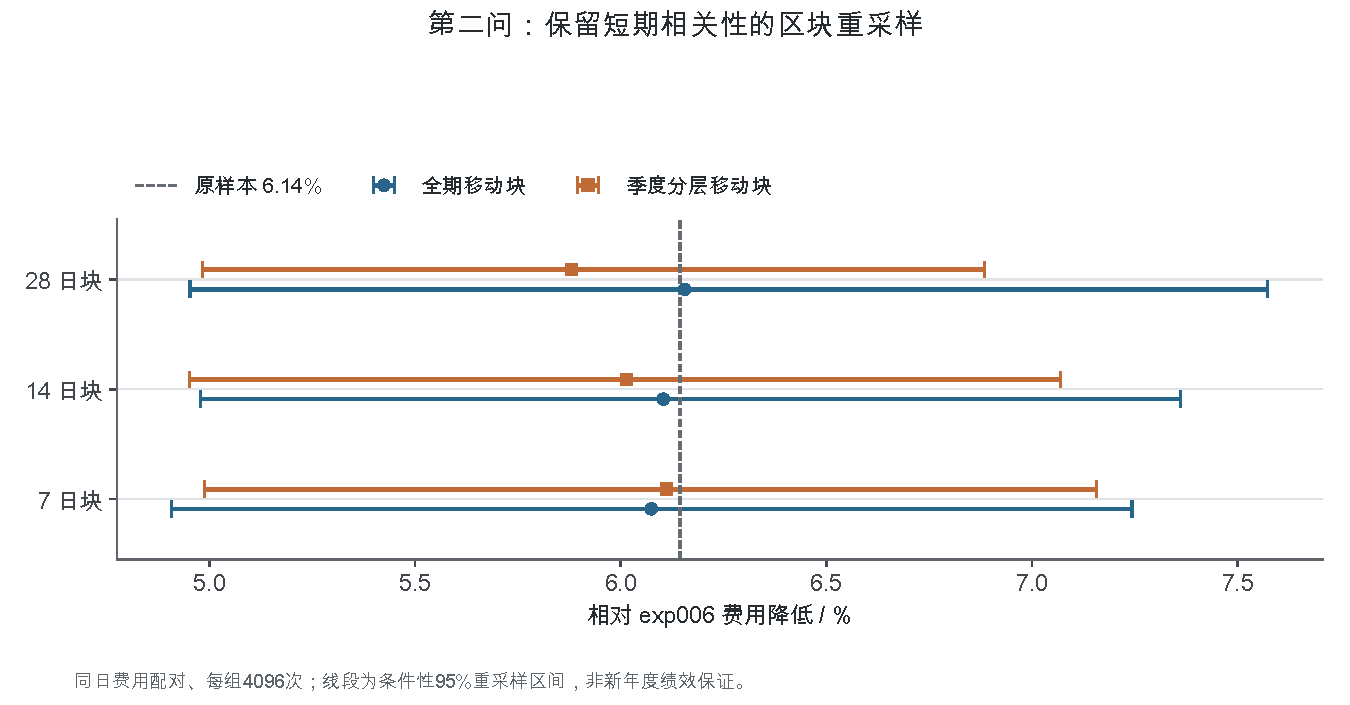
\includegraphics[width=0.96\linewidth]{../paper/figures/exp008_robustness/08_block_bootstrap.pdf}
  \caption{第二问：保留短期相关性的区块重采样}
  \label{fig:exp008-08_block_bootstrap}
\end{figure}

\begin{figure}[htbp]
  \centering
  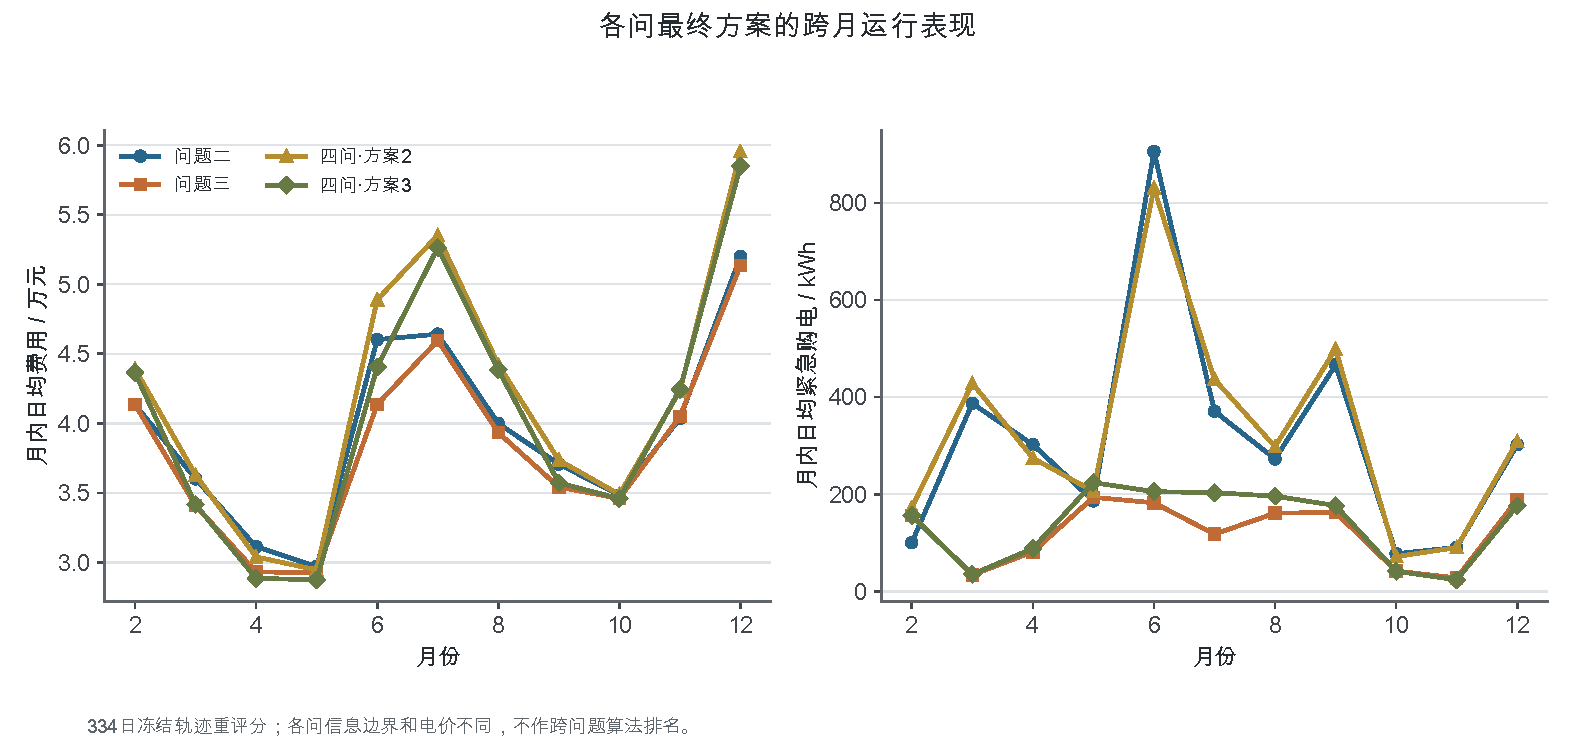
\includegraphics[width=0.96\linewidth]{../paper/figures/exp008_robustness/09_all_scenarios_monthly.pdf}
  \caption{各问最终方案的跨月运行表现}
  \label{fig:exp008-09_all_scenarios_monthly}
\end{figure}

\begin{figure}[htbp]
  \centering
  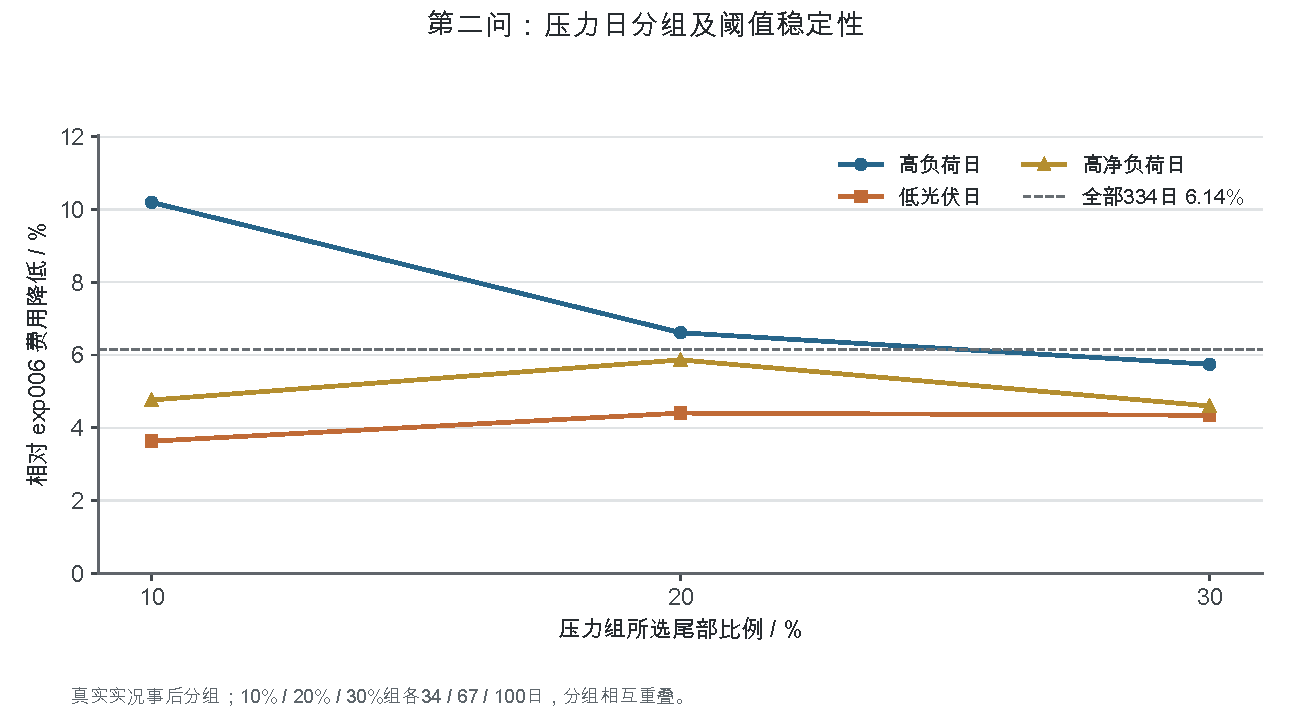
\includegraphics[width=0.96\linewidth]{../paper/figures/exp008_robustness/10_observed_stress_groups.pdf}
  \caption{第二问：压力日分组及阈值稳定性}
  \label{fig:exp008-10_observed_stress_groups}
\end{figure}

\begin{figure}[htbp]
  \centering
  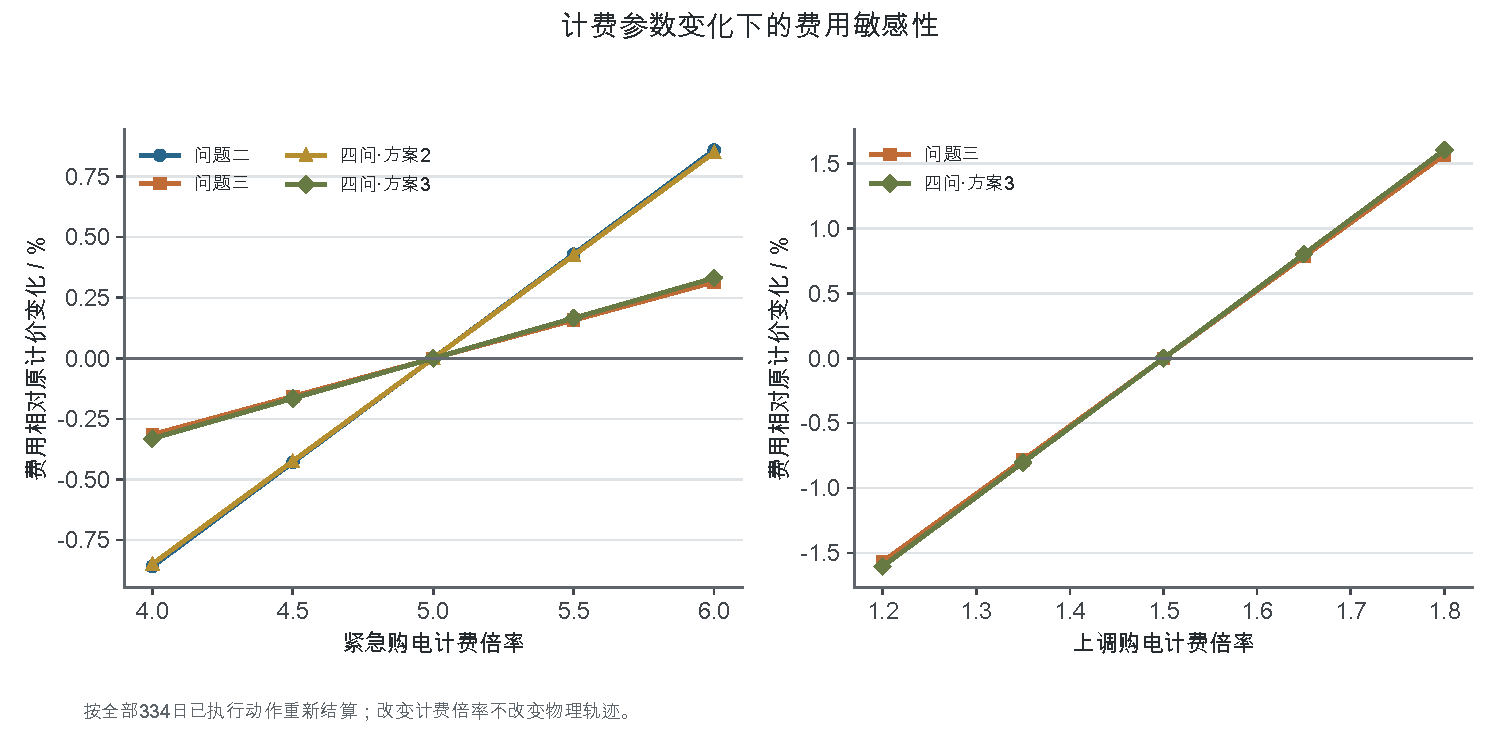
\includegraphics[width=0.96\linewidth]{../paper/figures/exp008_robustness/11_billing_sensitivity.pdf}
  \caption{计费参数变化下的费用敏感性}
  \label{fig:exp008-11_billing_sensitivity}
\end{figure}

\begin{figure}[htbp]
  \centering
  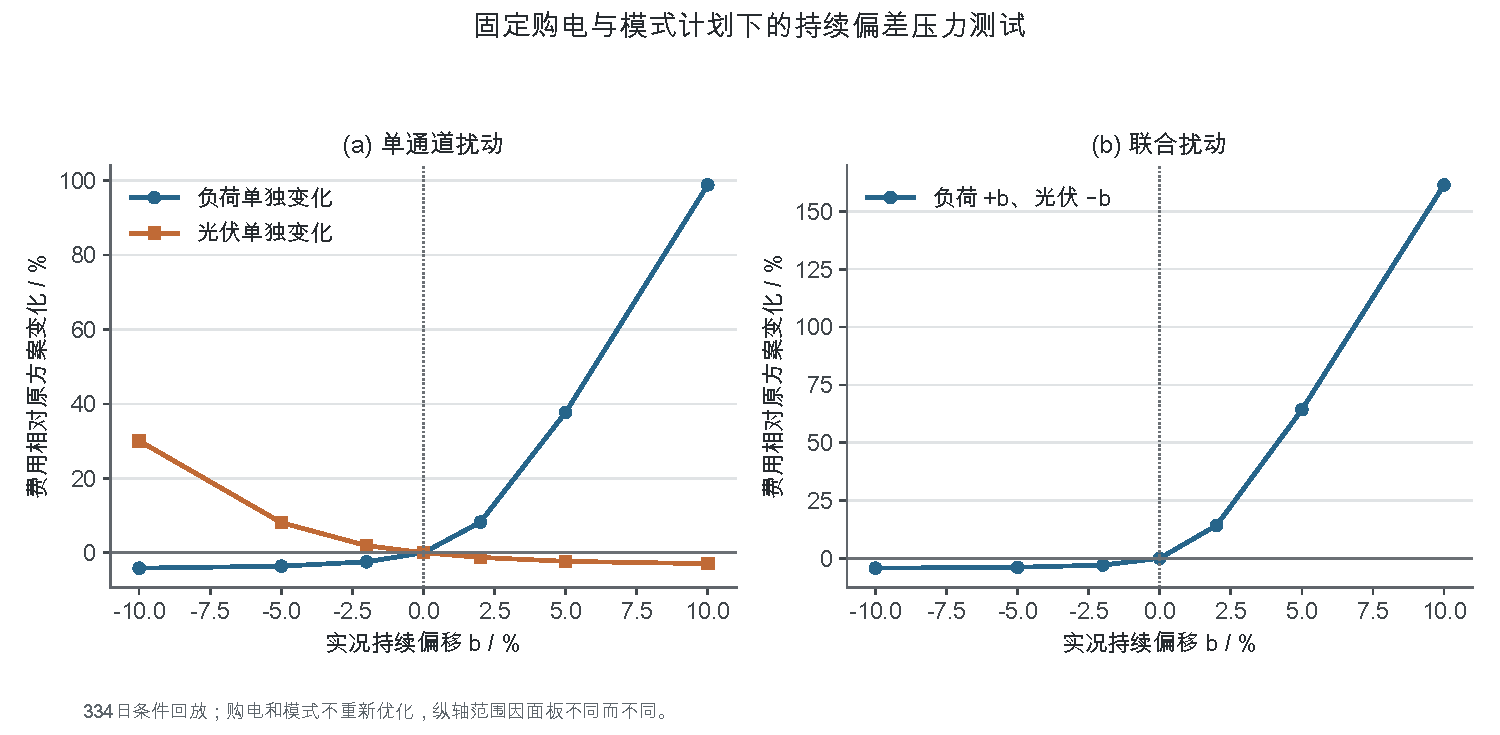
\includegraphics[width=0.96\linewidth]{../paper/figures/exp008_robustness/12_execution_bias.pdf}
  \caption{固定购电与模式计划下的持续偏差压力测试}
  \label{fig:exp008-12_execution_bias}
\end{figure}

\begin{figure}[htbp]
  \centering
  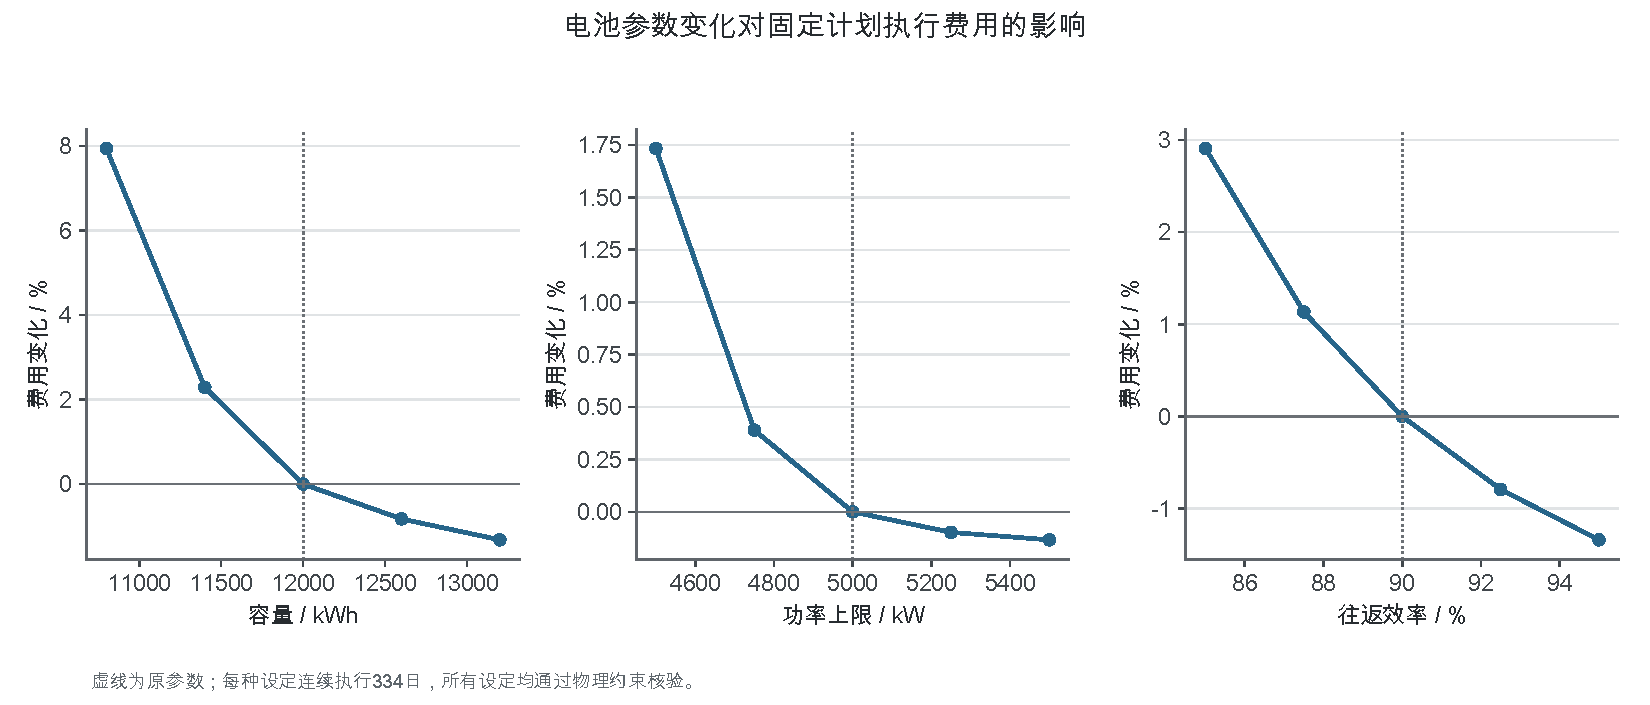
\includegraphics[width=0.96\linewidth]{../paper/figures/exp008_robustness/13_hardware_sensitivity.pdf}
  \caption{电池参数变化对固定计划执行费用的影响}
  \label{fig:exp008-13_hardware_sensitivity}
\end{figure}

\begin{figure}[htbp]
  \centering
  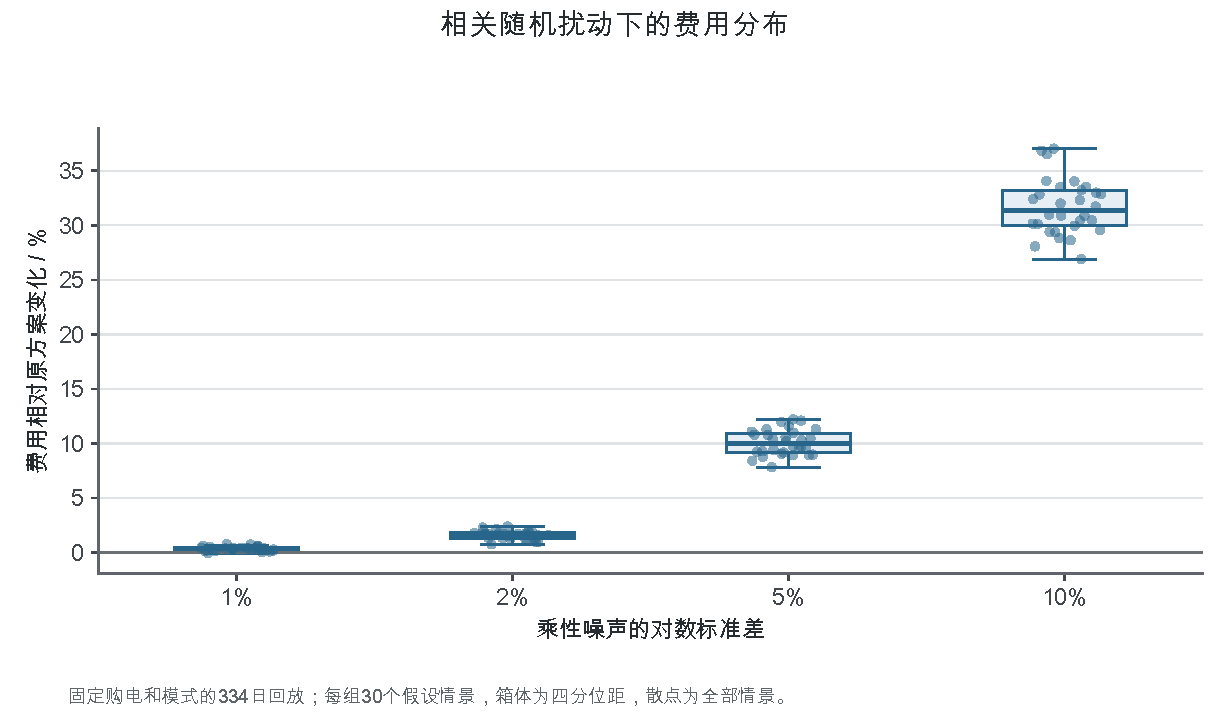
\includegraphics[width=0.96\linewidth]{../paper/figures/exp008_robustness/14_correlated_noise.pdf}
  \caption{相关随机扰动下的费用分布}
  \label{fig:exp008-14_correlated_noise}
\end{figure}

\begin{figure}[htbp]
  \centering
  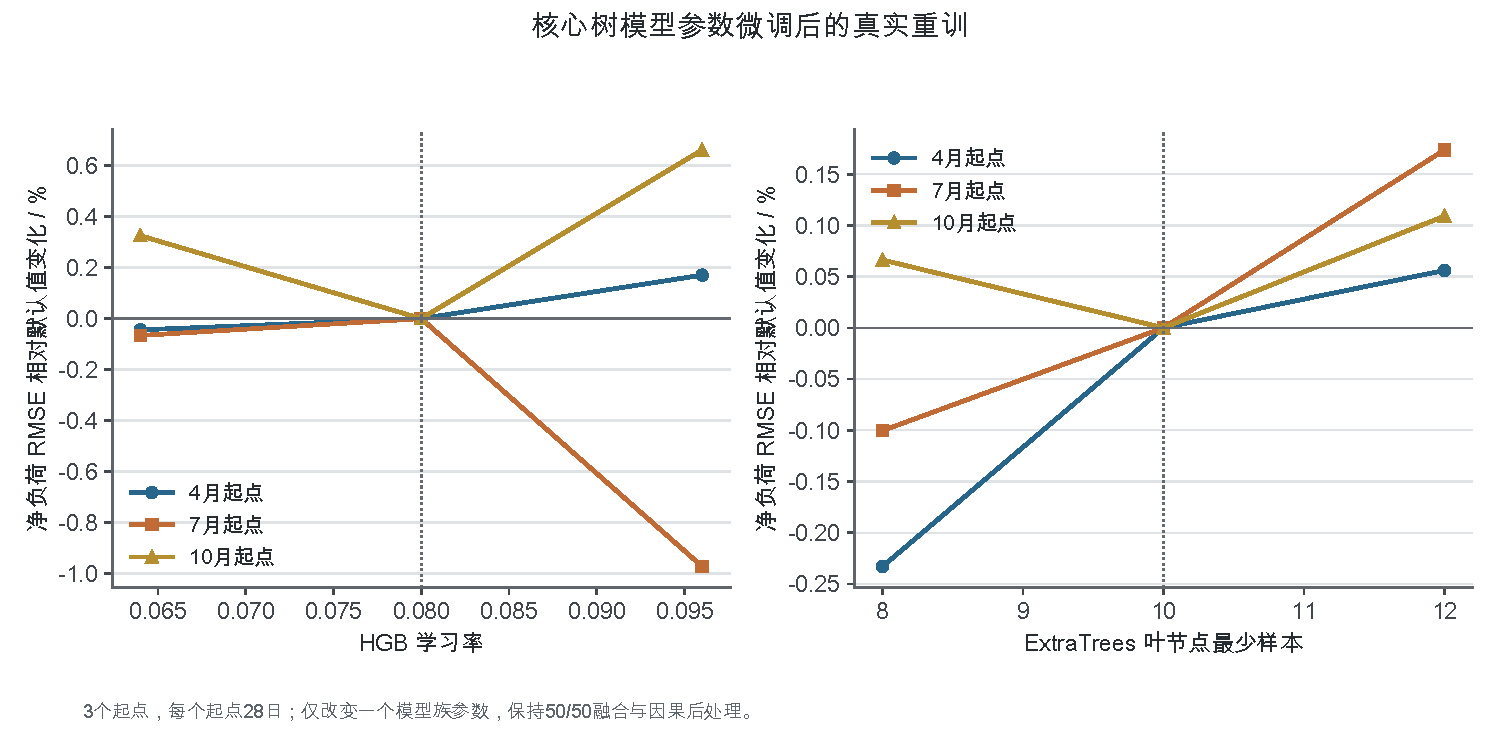
\includegraphics[width=0.96\linewidth]{../paper/figures/exp008_robustness/15_tree_hyperparameters.pdf}
  \caption{核心树模型参数微调后的真实重训}
  \label{fig:exp008-15_tree_hyperparameters}
\end{figure}
